
%\setcounter{chapter}{30}
\chapter{Deep generative models}\label{chapter:generative_models}

Generative models perform (or describe) the synthesis of data. Recall the image classifier from Chapter \ref{chapter:intro_to_learning}:

\begin{figure}[h]
    \centering
    \includegraphics[width=0.7\linewidth]{./figures/generative_models/image_classification.pdf}
    \label{fig:gen_models_image_classification}
\end{figure}

A generative model does the opposite:

\begin{figure}[h]
    \centering
    \hspace*{0.0\linewidth}\includegraphics[width=0.7\linewidth]{./figures/generative_models/image_generation.pdf}
    \label{fig:gen_models_image_generation}
\end{figure}

Whereas an image classifier is a function $f: \mathcal{X} \rightarrow \mathcal{Y}$, a generative model is a function in the opposite direction $g: \mathcal{Y} \rightarrow \mathcal{X}$. Things are a bit different in this direction. The function $f$ is {\bf many-to-one}: there are many images that all should be given the same label ``fish". The function $g$, on the other hand, is {\bf one-to-many}: there are many possible outputs for any given input. Generative models handle this ambiguity by making $g$ a {\bf stochastic function}. One way to make a function stochastic is to make it a deterministic function of a stochastic input: $g: \mathcal{Z} \times \mathcal{Y} \rightarrow \mathcal{X}$, with $\mathbf{z} \sim p(\mathbf{z})$, $\mathbf{z} \in \mathcal{Z}$. Often, we use Gaussian noise as the stochastic input: $p(\mathbf{z}) = \mathcal{N}(\mathbf{0},\mathbf{1})$:

\begin{figure}[h]
    \centering
    \hspace*{0.20\linewidth}\includegraphics[width=0.7\linewidth]{./figures/generative_models/image_generation_with_z.pdf}
    \label{fig:image_generation_with_z}
\end{figure}

Sometimes we wish to simply make up data from scratch -- in fact this is the canonical setting in which generative models are often studied. To do so, we can simply drop the dependency on the input label $y$. This yields a procedure for making data sampled as:
\begin{align}
    \mathbf{z} \sim p(\mathbf{z})\\
    \hat{\mathbf{x}} = g(\mathbf{z})
\end{align}
\marginnote{Corresponds to this graphical model:\\
\medbreak
    \centering
    \includegraphics[width=0.2\linewidth]{./figures/generative_models/graphical_model_z_to_x.pdf}
}[-2.1cm]
%This defines $\mathbf{x}$ as a random variable constructed by transforming random noise $\mathbf{z}$ through a deterministic function $g$. 
%In this form of generative modeling, our goal is to learn $g$ such that the distribution of random variable $\mathbf{x}$ matches some target distribution.
We call this an \textbf{unconditional generative model} because it is model of the unconditional distribution $p(\mathbf{x})$. Generally we will refer to unconditional generative models simply as ``generative models" and use the term \textbf{conditional generative model} for any model of the conditional distribution $p(\mathbf{x} | \mathbf{y})$.

Why bother with (unconditional) generative models, which make up random synthetic data? At first this may seem a silly goal. Why should we care to make up images from scratch? One reason is \emph{content creation}; we will see other reasons later, but content creation is a good starting point. Suppose we are making a video game and we want to automatically generate a bunch of exciting levels for the player the explore. We would like a procedure for making up new levels from scratch. Such {\bf procedural graphics} have been successfully used to generate random landscapes for game levels~\cite{XX}. Suppose we want to add a river to a landscape. We need to decide what path the river should take. A simple program for generating the path could be ``walk an increment forward, flip a coin to decide whether to turn left or right, repeat." Here is that program in pseudocode:
%Here is a simple program that can make the decisions for us, automating the generation of river paths:

\begin{algorithm}[h]
\label{finetuning_two_stage}
\SetAlgoVlined
\DontPrintSemicolon
\caption{Generative model of images of rivers}
{\bf Input:} Random vector of coin flips $\mathbf{z} = [z_0, \ldots, z_N]$ with each $z_i \in \{0,1\}$\;
{\bf Output:} Picture of a river\;
\texttt{start drawing at origin with heading = $90^\circ$}\;
\For{\upshape $i= 1, \dots, N$} {
    \texttt{extend line 1 unit in current heading direction}\;
    \If {$z_i==1$} {
        \texttt{rotate heading $10^\circ$ to the right}
    }
    \Else {
        \texttt{rotate heading $10^\circ$ to the left}
    }
}
\end{algorithm}

Here are a few rivers this program draws:
\begin{figure}[h]
    \centering
    \includegraphics[width=0.8\linewidth]{./figures/generative_models/G4_river.pdf}
    \label{fig:generative_models:rivers1}
\end{figure}

This program relies on a sequence of random coin flips to generate the path of the river. In other words, the program took a sequence of flips as input, and converted this ``noise" to a image of the path of the river. It's exactly the same idea as we described above for generating images of fish, just this time the generator is a program that makes rivers:
\begin{figure}[h]
    \centering
    \includegraphics[width=0.7\linewidth]{./figures/generative_models/gen_model_of_rivers_diagram.pdf}
    \label{fig:generative_models:gen_model_of_rivers_diagram}
\end{figure}

This generator was written by hand. Next we will see generative models that \textit{learn} the program that synthesizes data.%, by setting its parameters such that the output matches some target distribution, for example, we may wish the output to match the distribution of actual river paths in the wild.
%Imagination.

\section{Learning generative models}

\subsection{Data generators}
How can we learn to synthesize images that look realistic? The machine learning way to do this is to start with a training set of \textit{examples} of real images, $\{\mathbf{x}^{(i)}\}_{i=1}^N$. Recall that in supervised learning, an example was defined as an \{\texttt{input}, \texttt{output}\} pair; here things are actually no different, only the \texttt{input} happens to be the null set. We feed these examples to a learner, which spits out a \textbf{generator} function. Later, we may query the generator with random noise source $\mathbf{z}$ to produce novel outputs, a process called sampling from the model:
\begin{figure}[h]
    \centering
    \includegraphics[width=0.75\linewidth]{./figures/generative_models/gen_model_training_vs_sampling.pdf}
    \label{fig:generative_models:gen_model_training_vs_sampling}
    \caption{Learning and using a generator.}
\end{figure}

The objective of the learner is to create a generator that produces synthetic \textbf{fake} data, $\{\hat{\mathbf{x}}^{(i)}\}_{i=1}^N$, that ``looks like" the \textbf{real} data, $\{\mathbf{x}^{(i)}\}_{i=1}^N$. There are a lot of ways of define ``looks like'' and they each result in a different kind of generative model. Two examples are:
\begin{enumerate}
    \item Fake data looks like real data if matches the real data in terms of certain marginal statistics, e.g., it has the same mean color as real photos, or the same color variance, or the same edge statistics, etc.
    \item Fake data looks like real data if it has high probability under a density model fit to the real data.
\end{enumerate}
The first approach is the one we saw in Chapter XX on statistical image models, where fake textures were made that had the same filter response statistics as a real training example. This approach works well when we only want to match certain properties of the training data. The second approach, which is the main focus of this chapter, is better when we want to produce fake data that matches \textit{all} properties of the training examples.

To be precise, the goal of the deep generative models we consider in this chapter is to produce fake data that is \textit{identically distributed} as the training data, i.e. we want $\hat{\mathbf{x}} \sim p_{\texttt{data}}$ where $p_{\texttt{data}}$ is the true process that produced the training data. We will see several ways to achieve this in the following sections.

\subsection{Density models}
Some generative models not only produce generators but also yield a probability density function $p_{\theta}: \mathcal{X} \rightarrow [0,1]$ fit to the training data. This density function may play a role in training the generator (e.g., we want the generator to produce samples from $p_{\theta}$) or the density function may be the goal itself (e.g., we want to be able to estimate the probability of datapoints in order to detect anomalies).

Other generative models \textit{only} produce a density $p_{\theta}$ and do not learn any explicit generator function. Instead, samples can be down from $p_{\theta}$ using procedures such as \textbf{Markov Chain Monte Carlo} (\textbf{MCMC}).

%Generative models that just produce a generator $G_{\theta}: \mathcal{Z} \rightarrow \mathcal{X}$ are sometimes called {\bf implicit generative models}, because they do not explicitly give us the likelihood (a.k.a. probability) of the samples they generate. Other generative models instead fit an explicit probability {\bf density} to the input data, $p_{\theta}: \mathcal{X} \rightarrow [0,1]$:\marginnote{It's unfortunate that history chose the term ``implicit" for generative models that give samples but not densities, and ``explicit" for generative models that give densities but not samples. We feel it would make more sense to swap the terms, and think of density models as implicitly defining a way of generating data, and samplers as explicitly defining a way of generating data, but alas that's not the accepted vocabulary.}[-1.3cm]

%A classical way to learn a generative model is to first fit a probability density function to the training data, then sample from this density. In 
%In this case, the ``Generator" in Figure \ref{fig:generative_models:gen_model_training_vs_sampling} is actually a program that repeatedly calls a density function as a subroutine. Sometimes the learned density model is itself called a generative model since it implicitly defines a way to generate data.\maginnote{Confusingly, generative models that skip the step of modeling a density function as sometimes called ``implicit" models, because the density is implied rather than explicit.}


%If we are given training data $\mathbf{x} \sim p_{\texttt{data}}$, our goal is to learn a {\bf generator} $G_{\theta}$ from this data such that $G_{\theta}$ produces synthetic data, $\hat{\mathbf{x}}$ that \textit{looks like the training data}. There are a lot of ways of define ``looks like'' and they each result in a different kind of generative model.

%We will define the function that checks if the outputs of a generator ``look like" the training data to be called a {\bf critic}. \marginnote{``Critic" is not a standard term in in this context; we are borrowing it from ``actor-critic" methods in reinforcement learning. In the context of generative models, the actor is the generator and the critic is either a likelihood function, an energy function, or a discriminator function, depending on the type of model.} The critic takes one or more generated images as input and scores them; we call images output by the generated as \textbf{fake} images, and those sampled from the training data as \textbf{real} images. The goal of the generator is to produce images that score highly under the critic, and the goal of the critic is to assign high scores to realistic images. In Chapter XX, we already saw one example of a generator and a critic: the Heeger \& Bergen model uses a critic that checks if a fake texture has the same filter response statistics as a real texture example. The generator is then a procedure that iteratively projects random noise into the subspace with features that satisfy the critic.

%The first thing to note is that we do not, typically, care to make fake images that are exact copy of the training data, identical in every way. Instead, we want to make fake data that matches some desired properties of the training data, but is otherwise randomized. Generically, therefore, the critic should not check if the fake images are identical to training images but instead that they match certain desired properties or statistics of the training data. For example, we may want to produce fake images that have the same \textit{mean} and \textit{variance} as the training data. 

%The most popular kinds of generative models aim to make synthetic data that has the same \textit{distribution} as the training data. For these models, one standard kind of critic is a density function. First we fit the density to the training data, then we sample from that density.

%The ``looks like" comparator is called a ``critic". The critic scores if an image has the same statistical properties as the training data, for example if it is likely to have come from the same distribution as the training data.

%Most generative models consist of two functions: a {\bf generator} and a {\bf critic}.\marginnote{``Critic" is not a standard term in in this context; we are borrowing it from ``actor-critic" methods in reinforcement learning. In the context of generative models, the actor is the generator and the critic is either a likelihood function, an energy function, or a discriminator function, depending on the type of model.} The critic is a function that checks if a candidate set of images is a set we like. The generator is a function that tries to make candidate images the critic will score highly.

%\marginnote{This is actually a common setup, often we have f* = argmin_f V(f), where V is a critic that evaluates how good a function is. We can either first learn V, then use optimization to get f*, or we can directly learn f* or can learn both simultaneously.}

%How can we learn to do this? If we are given training data $\mathbf{x} \sim p_{\texttt{data}}$, our goal is to learn $G_{\theta}$ from this data such that $G_{\theta}$ produces synthetic data, $\hat{\mathbf{x}}$ that \textit{looks like the training data}. There are a lot of ways of define ``looks like'' and they each result in a different kind of generative model. 

%The first thing to note is that we do not, typically, care to make synthetic data that is just an exact copy of the training data, identical in every way. Instead, we will make synthetic data that matches some desired properties of the training data, but is otherwise randomized. Generically, the desired properties will be summary statistics of the training data. For example, we may want to produce synthetic data that has the same \textit{mean} and \textit{variance} as the training data. The most popular kinds of generative models aim to make synthetic data that has the same \textit{distribution} as the training data.  %Remember, the distribution of the training data is a summary statistic of it. 
%Formally, we want our model to produce samples that are identically distributed as the training data, i.e. $\hat{\mathbf{x}} \sim p_{\texttt{data}}$:\footnote{the figures on this page and the next are derived from: \texttt{http://introtodeeplearning.com/materials/2019\_6S191\_L4.pdf}}

%\begin{figure}[h]
%    \centering
%    \includegraphics[width=0.9\linewidth]{./figures/generative_models/sampler_formalism.pdf}
%    \label{fig:sampler_formalism}
%\end{figure}

%Generative models that just produce a {\bf sampler} $G_{\theta}: \mathcal{Z} \rightarrow \mathcal{X}$ are sometimes called {\bf implicit generative models}, because they do not explicitly give us the likelihood (a.k.a. probability) of the samples they generate. Other generative models instead fit an explicit probability {\bf density} to the input data, $p_{\theta}: \mathcal{X} \rightarrow [0,1]$:\marginnote{It's unfortunate that history chose the term ``implicit" for generative models that give samples but not densities, and ``explicit" for generative models that give densities but not samples. We feel it would make more sense to swap the terms, and think of density models as implicitly defining a way of generating data, and samplers as explicitly defining a way of generating data, but alas that's not the accepted vocabulary.}[-1.3cm]

%A generative model \emph{learner} takes data $\{\mathbf{x}_i\}_{i=1}^N$ as input and outputs one of two things (or sometimes both): 1) a {\bf density} $p_{\theta}: \mathcal{X} \rightarrow [0,1]$, 2) a {\bf sampler} $g_{\theta}: \mathcal{Z} \rightarrow \mathcal{X}$ that maps random noise $z$ to data sample $x$, i.e. $x = g(z)$, $z \sim p(z)$, such that $x \sim p_{\texttt{data}}(x)$:

% \begin{figure}[h]
%     \centering
%     \includegraphics[width=0.9\linewidth]{./figures/generative_models/density_modeling_formalism.pdf}
%     \label{fig:density_modeling_formalism}
% \end{figure}

The objective of the learner for a density model is to output a density function $p_{\theta}$ that is as close as possible to $p_{\texttt{data}}$. How should we measure closeness? We need to define a {\bf divergence} between two distributions, $D$, which yields the following optimization problem:
\begin{equation}
    \argmin_{p_\theta} D(p_{\theta}, p_{\texttt{data}})
\end{equation}
A problem is that we do not actually have the function $p_{\texttt{data}}$, we only have samples from this function, $\mathbf{x} \sim p_{\texttt{data}}$. Therefore, we need a divergence $D$ that measures the ``distance"\footnote{The divergence need not be a proper distance \emph{metric}, and often is not; it can be non-symmetric, where $D(p,q) \neq D(q,p)$, and need not satisfy the triangle-inequality. In fact, a divergence is defined by just two properties, non-negativity and $D(p,q) = 0 \iff p=q$.} between $p_{\theta}$ and $p_{\texttt{data}}$ while only accessing samples from $p_{\texttt{data}}$. A common choice is to use the ``forward" {\bf KL-divergence}, which is defined as follows:
\begin{align}
    p_{\theta}^* &= \argmin_{p_\theta} \texttt{KL}(p_{\texttt{data}}, p_{\theta})\\
    &= \argmin_{p_\theta} \mathbb{E}_{\mathbf{x} \sim p_{\texttt{data}}}[\log \frac{p_{\theta}(\mathbf{x})}{p_{\texttt{data}}(\mathbf{x})}]\\
    &= \argmin_{p_\theta} \mathbb{E}_{\mathbf{x} \sim p_{\texttt{data}}}[\log p_{\theta}(\mathbf{x})] - \mathbb{E}_{\mathbf{x} \sim p_{\texttt{data}}}[\log p_{\texttt{data}}(\mathbf{x})]\\
    &= \argmin_{p_\theta} \mathbb{E}_{\mathbf{x} \sim p_{\texttt{data}}}[\log p_{\theta}(\mathbf{x})] \quad\quad \triangleleft{\text{dropped 2nd term since no dependence on $p_{\theta}$}} \label{eqn:generative_models:max_likelihood}\\
    &\approx \argmin_{p_\theta} \frac{1}{N} \sum_{i=1}^N \log p_{\theta}(\mathbf{x}^{(i)})
\end{align}
where the final line is an empirical estimate of the expectation by sampling over the training dataset $\{\mathbf{x}^{(i)}\}_{i=1}^N$. Equation \ref{eqn:generative_models:max_likelihood} is the \emph{expected log likelihood of the training data under the model's density function}. Maximizing this objective is therefore a form of {\bf max likelihood learning}. 

\subsection{Energy-based models}
Density models constrain the learned function to be normalized, i.e. $\int_{\mathbf{x}} p_{\theta}(\mathbf{x})d\mathbf{x} = 1$. This constraint is often hard to realize. For example, one approach is to learn an unnormalized function $E_{\theta}$, then convert it to the normalized density $p_{\theta} = \frac{E_{\theta}}{Z}$, where $Z = \int_{\mathbf{x}} p_{\mathbf{x}}d\mathbf{x}$ is the normalizing constant. $Z$ can be very expensive to compute and often can only be approximated.

\textbf{Energy-based models} (\textbf{EBM}s) address this by simply skipping the step where we normalize the density, and letting the output of the learner just be $E_\theta$. Eventhough it is not a true probability density, $E$ can still be used for many of the applications we would want a density for. This is because we can compare \textit{relative probabilities} with $E_\theta$ since $\frac{E_\theta(\mathbf{x}_1)}{E_\theta(\mathbf{x}_2)} = \frac{p_\theta(\mathbf{x}_1)}{p_\theta(\mathbf{x}_2)}$. Knowing relative probabilities is all that is required for MCMC sampling algorithms, for certain kinds of outlier detection, for maximizing the probability of a datapoint $\mathbf{x}$, and so on.


\newpage
Some generative models give density or energy functions, others give generator functions, and still others give both. We can summarize all these kinds of models with the following learning diagram: %The kinds of {\bf deep generative models} that are popular these days, have the following form:
\begin{center}
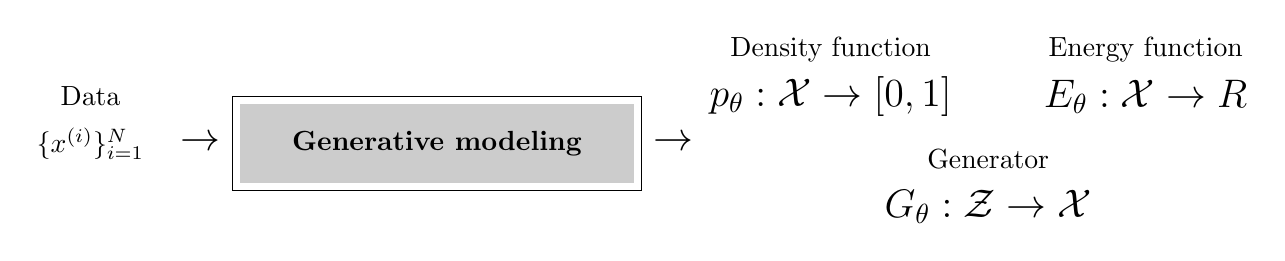
\begin{tikzpicture}
    \draw (0,1.2) rectangle (5.2,2.4); % outer box
    \fill[black!20] (0.1,1.3) rectangle (5.1,2.3); % gray box
    \node[] at (2.6,1.8) {{\bf Generative modeling}};
    \node[] at (-1.8,2.4) {Data};
    \node[] at (-1.8,1.8) {$\{x^{(i)}\}_{i=1}^N$};
    \node[] at (-0.4,1.8) {{\Large  $ \rightarrow$}};
    \node[] at (7.6,3.0) {Density function};
    \node[] at (7.6,2.4) {{\Large $p_{\theta}: \mathcal{X} \rightarrow [0,1]$}};
    \node[] at (11.6,3.0) {Energy function};
    \node[] at (11.6,2.4) {{\Large $E_{\theta}: \mathcal{X} \rightarrow \mathbb{R}$}};
    \node[] at (9.6,1.6) {Generator};
    \node[] at (9.6,1.0) {{\Large $G_{\theta}: \mathcal{Z} \rightarrow \mathcal{X}$}};
    \node[] at (5.6,1.8) {{\Large  $ \rightarrow$}};
\end{tikzpicture}
\end{center}


% \begin{figure}[h]
%     \centering
%     \includegraphics[width=0.8\linewidth]{./figures/generative_models/deep_generative_model_formalism.pdf}
%     \label{fig:deep_generative_model_formalism}
% \end{figure}

\section{Types of deep generative models {\small[Advanced Topics]}}

% \begin{table}[]
%     \centering
%     \begin{tabular}{c|c|c}
%         Method & Generator & Critic \\
%         \hline
%         GAN & Neural net: $G_{\theta}: \mathcal{Z} \rightarrow \mathcal{X}$ & Neural net $D_{\phi}: \mathcal{X} \rightarrow \mathbb{R}$\\
%         EBM & MCMC & Neural net $E_{\theta}:\mathcal{X} \rightarrow \mathbb{R}$ \\
%         Normalizing flow & Neural net $G_{\theta}: \mathcal{Z} \rightarrow \mathcal{X}$ & Density $p_{\theta}: \mathcal{X} \rightarrow [0,1], p_{\theta}(\mathbf{x}) = p_{\mathbf{z}}(G_{\theta}^{-1}(\mathbf{x}))|\det(\frac{\partial G_{\theta}^{-1}(\mathbf{x})}{\partial \mathbf{x}})|$ \\
%         VAE & Neural net: $G_{\theta}: \mathcal{Z} \rightarrow \mathcal{X}$ & Reconstruction error: $\mathcal{X} \rightarrow \mathbb{R}, \norm{G_{\theta}(F_{\phi}(\mathbf{x}))-\mathbf{x}}$\\
%         Autoregressive & Ancestral sampling & Density $p_{\theta}: \mathcal{X} \rightarrow [0,1], p_{\theta}(\mathbf{x}) = \prod_i p_{\theta}(x_i | x_1, \ldots, x_{i-1})$ & \\
%     \end{tabular}
%     \caption{}
%     \label{tab:my_label}
% \end{table}

The field of deep generative modeling is rapidly evolving. We will next cover five families of model that are currently popular, but if you are reading this in a few years, it's likely a whole host of new models will exist. The important thing to notice is how all these models stem from the same ingredients, just used in slightly different proportions and combinations. As you read these sections look for the commonalities. For example, which of the models are optimizing a likelihood function? Which are based on a factorization of a joint probability distribution. Which use sampling to approximate intractable integrals? And so forth. The next generation of models will likely be minor variations on these themes, just as this generation of models can be viewed as minor variations on older models.% from the fields of statistics~\cite{XX}, physics~\cite{XX}, and economics~\cite{XX}.

\subsection{Autoregressive models}
We will start with a very simple and intuitive model, where we synthesize images by sampling pixels one by one. Each new pixel is decided on based on the sequence already generated. Such an approach is called an {\bf autoregressive model}. These are max likelihood models: they learn a distribution over pixels that maximizes the density assigned to observed pixels in the training data. 

These models can be easily understood by first considering the problem of modeling one pixel, then two, and so on. The first observation to make is that it's pretty easy to model a single grayscale pixel. Such a pixel can take on 256 possible values. So it suffices to use a categorical distribution to represent the probability that the pixel takes on each of these possible values. The categorical distribution is fully expressive: any possible pmf over the 256 values can be represented with the categorical distribution. Fitting this categorical distribution to training data just amounts to counting how often we observe each of the 256 values in the training pixels, and normalizing by the total number of training pixels. So we know how to model one grayscale pixel. %Autoregressive models just do this over and over for all the pixels.

\begin{table}[t]
    \centering
    \begin{tabular}{c|c|c|c}
        Method & Explicit latents? & Explicit density? & Explicit generator? \\
        \hline
        Normalizing flow & \checkmark (high-dimensional) & \checkmark & \checkmark \\
        VAE & \checkmark & & \checkmark \\
        GAN & \checkmark & & \checkmark \\
        Autoregressive models &  & \checkmark & \\
        Energy-based model &  & \checkmark (unnormalized) & \\
    \end{tabular}
    \caption{Three desirable properties in a generative model. No method achieves all three (without caveats). VAEs and GANs are good at representation learning (i.e. at finding a low-dimensional latent space). Normalizing flows and autoregressive models are great if you want to estimate the likelihood of your data points (e.g., for anomaly detection). Energy-based models can be an especially efficient way to model an unnormalized density.}
    \label{tab:types_of_gen_model}
\end{table}

How do we model the distribution over a second grayscale pixel given the first? In fact, we already know how to model this setting; mathematically, we are just trying to learn $p(y | \mathbf{x})$ where $\mathbf{x}$ is some arbitrary information we condition on and $y$ is a scalar categorical variable. This is exactly what softmax regression does, which we saw in Chapter \ref{chapter:intro_to_learning}). In that chapter we were modeling a $K$-way categorical distribution over $K$ object classes, conditioned on an input image. Now we can use exactly the same tools to model a $256$-way distribution over a the second pixel in a sequence conditioned on the first.

What about the third pixel, conditioned on the first two? Well, this is again a problem of the form $p(y | \mathbf{x})$ where $\mathbf{x}$ is arbitrary and $y$ is a categorical variable! So this is yet another softmax regression problem. Now you can see the induction: modeling each next pixel in the sequence that forms the image is a softmax regression problem.

%The hard part is to model a structured joint distribution over $\mathbf{y} = [y_1, \ldots, y_n]$. 

What we have done here is to exploit the {\bf chain rule of probability}. This rule allows us to factorize \textit{any} joint distribution into a product of conditionals as follows:
\begin{align}
    p(\mathbf{x}) &= p(x_n | x_1, \ldots, x_{n-1})p(x_{n-1} | x_1, \ldots, x_{n-2}) \quad \ldots \quad p(x_2|x_1)p(x_1)\\
    p(\mathbf{x}) &= \prod_{i=2}^n p(x_i | x_1, \ldots, x_{i-1})p(x_1)\label{eqn:generative_models:autoregressive_likelihood}
\end{align}

Now that's just a sequence of univariate predictions. So we have reduced the problem of modeling a joint distribution into a sequence of problems of modeling a single output variable, and that's a problem we know how to solve.

Autogressive models give us an explicit density function, Equation \ref{eqn:generative_models:autoregressive_likelihood}. To sample from this density we can use {\bf ancestral sampling}, which refers to sampling the first pixel from $p(x_1)$, then, conditioned on this pixel, sample the second from $p(x_2|x_1)$ an so forth. Since each of these densities is a categorical distribution, sampling is easy: one option is to partition a unit line segment into regions of length equal to the categorical probabilities and see where a uniform random draw along this line falls. Autogressive models do not have latent variables $\mathbf{z}$, which makes them incompatible with applications that involve extracting or manipulating latent variables.

%\paragraph{Nonparametric texture synthesis is an autoregressive model}


\subsection{Normalizing flows}

Next we will consider generative models with latent variables, $\mathbf{z}$. The models we will cover are implicit: they learn a generator which maps a base distribution over $\mathbf{z}$ to a transformed distribution over $\mathbf{x}$. Typically the base distribution is something simple like $p_{\mathbf{z}} = \mathcal{N}(0,1)$ and the mapping is a deep neural net. The difference between different methods is mainly in the learning objective, which encourages this mapping to fit the data distribution.

We will start with two implicit max likelihood models, normalizing flows and variational autoencoders. These models share the same objective as autoregressive models -- assign maximum probability density to the training datapoints -- but differ in how they achieve this. For max likelihood models, we need to calculate or approximate the data likelihood function, $L(\{\mathbf{x}^{(i)}\}_{i=1}^N, \theta)$, but how we calculate likelihood can be done in a few ways. In explicit density models, like autoregressive models, we directly learn the likelihood function: $L(\{\mathbf{x}^{(i)}\}_{i=1}^N, \theta) = \prod_i p_{\theta}(\mathbf{x}^{(i)})$. Then we adjust the parameters to maximize this quantity.

In implicit models, things are a bit harder since we don't have an explicit likelihood function. Instead we learn a generator $G_{\theta}$. If the sampler is bijective, so that $G^{-1}$ exists and can be computed, things are actually still easy. We can use the {\bf change of variables} formula to compute the likelihood of data implied by our sampler:
\begin{equation*}
    L(\mathbf{x}, \theta) = p_{\mathbf{z}}(G_{\theta}^{-1}(\mathbf{x}))|\det(\frac{\partial G_{\theta}^{-1}(\mathbf{x})}{\partial \mathbf{x}})| 
\end{equation*}
%where $p_{\mathbf{z}}$ is our prior (usually a Normal distribution or uniform distribution).

Max likelihood learning corresponds to maximizing the log likelihood of the training data, $\{\mathbf{x}^{(i)}\}_{i=1}^N$, so here it looks like:
\begin{equation}
    \argmax_{G_{\theta}} \frac{1}{N} \sum_{i=1}^N \log p_{\mathbf{z}}(G_{\theta}^{-1}(\mathbf{x}^{(i)})) + \log |\det(\frac{\partial G_{\theta}^{-1}(\mathbf{x}^{(i)})}{\partial \mathbf{x}^{(i)}})|\label{eqn:generative_models:normalization_flows}
\end{equation}
{\bf Normalizing flows} are generative models learned using Equation \ref{eqn:generative_models:normalization_flows}. The name is a reference to the fact that the generator is bijective (a ``flow") and the latent variables have a known (``normalized") density they are drawn from.

%{\bf Diffusion models} are a kind of normalizing flow. They define an invertible process that adds noise to an image in a series of steps. With enough steps, the image because completely random noise. Because each step is invertible, the process can be reversed: first sample random noise, then step by step ``congeal" it into an image. <-- this is wrong, diffusion models are not bijective

\subsection{Variational Autoencoders}

If the mapping is not bijective, the change of variables formula does not apply. Instead, one option is to build up a density model, from our sampler, by putting a little blip of Gaussian probability around each image, $G_{\theta}(\mathbf{z}^{(i)})$, generated by our sampler. Commonly, we augment $G$ to also output the variance, $\sigma$, of this Gaussian, so we have $G^{\mu}_{\theta}$ and $G^{\sigma}_{\theta}$. This gives us an infinite mixture of Gaussians as our likelihood model: $L(\mathbf{x}, \theta) = \int_{\mathbf{z}} p_{\theta}(\mathbf{x} | \mathbf{z})p(\mathbf{z})d\mathbf{z}$, where $p_{\theta}(\mathbf{x} | \mathbf{z}) = \mathcal{N}(\mathbf{x}; G_{\theta}^{\mu}, G_{\theta}^{\sigma})$ and $p_{\mathbf{z}}$ is usually a unit Normal distribution.

%In the general case, we have $L(\mathbf{x}, \theta) = \int_\mathbf{z} \mathbbm{1}(\mathbf{x} = G_{\theta}(\mathbf{z}))p(\mathbf{z})d\mathbf{z}$. This integral is intractable. We can use the calculus of variations to approximate it. Commonly, we add some noise to $G_{\theta}(\mathbf{z})$, which makes the formulas differentiable.% (we will see this more clearly in just a bit).

This integral is usually very expensive to compute so we will approximate it, and this leads to a method called {\bf Variational Autoencoders} ({\bf VAEs}). The first trick in VAEs is to use a \textit{Monte Carlo estimate} of the integral:
\begin{align}
    L(\mathbf{x}, \theta) &= \int_{\mathbf{z}} p_{\theta}(\mathbf{x} | \mathbf{z})p(\mathbf{z})d\mathbf{z} \label{eqn:generative_models:vae_likelihood}\\
    &= \mathbb{E}_{\mathbf{z}\sim p(\mathbf{z})}[p_{\theta}(\mathbf{x} | \mathbf{z})]\\
    &\approx \frac{1}{N} \sum_{i=1}^N p_{\theta}(\mathbf{x} | \mathbf{z}^{(i)}), \quad \mathbf{z}^{(i)} \sim p(\mathbf{z})
\end{align}
So far so good, but for this to be a good approximation our number of samples, $N$, may need to be very large. Now here comes the real trick: \textit{try to only sample those $\mathbf{z}$'s that are actually responsible generating the observed $\mathbf{x}$, i.e. those $\mathbf{z}$'s for which $p_{\theta}(\mathbf{x}, \mathbf{z})$ is large}. The idea is that for most $\mathbf{z}$'s, $p_{\theta}(\mathbf{x}, \mathbf{z})$ will end up being near zero. This idea is called {\bf importance sampling}. Rather than sampling $\mathbf{z}^{(i)} \sim p(\mathbf{z})$ to approximate the integral, we sample from another distribution $\mathbf{z}^{(i)} \sim q(\mathbf{z})$, and multiply by a correction factor $\frac{p(\mathbf{z})}{q(\mathbf{z})}$ to account for the fact that we are sampling from a biased distribution:
\begin{align}
L(\mathbf{x}, \theta) &= \mathbb{E}_{\mathbf{z}\sim p(\mathbf{z})}\Big[p_{\theta}(\mathbf{x} | \mathbf{z})\Big] \label{eqn:generative_models:vae_likelihood2}\\
&= \mathbb{E}_{\mathbf{z}\sim q(\mathbf{z})}\Big[\frac{p(\mathbf{z})}{q(\mathbf{z})} p_{\theta}(\mathbf{x} | \mathbf{z})\Big]%\\
%&\approx \frac{1}{N} \sum_{i=1}^N \frac{p(\mathbf{z}^{(i)})}{q(\mathbf{z}^{(i)})} p_{\theta}(\mathbf{x} | \mathbf{z}^{(i)}), \quad \mathbf{z}^{(i)} \sim q(\mathbf{z})
\end{align}
As can be seen if you write out the integral, the two expectations above are \textit{exactly equal}, and this is true for \textit{any} distribution $q$. Intuitively, as we alluded to above, we want the samples from $q$ to be the dominate terms in the integral in Eqn. \ref{eqn:generative_models:vae_likelihood}, so that only a few samples will suffice to well approximate the integral. The theory of importance sampling tells us that indeed this is the optimal thing to do and in particular we should ideally set $q = p_{\theta}(\mathbf{z}|\mathbf{x})$, i.e. $q$ should be a prediction of exactly which $\mathbf{z}$ was responsible for generating the observed $\mathbf{x}$. 

Now we have a goal in mind for $q$: we want $q$ to be as close as possible to $p_{\theta}(\mathbf{z}|\mathbf{x})$. This way we will get the best estimate of the likelihood $L$ when we use that learned $q$. Note that since $q$ can be any distribution, it can, for instance, be a distribution conditioned on $\mathbf{x}$, and that's what we will use so as to best approximate $p_{\theta}(\mathbf{z}|\mathbf{x})$, since it is also conditioned on $\mathbf{x}$. Further, because we are learning parameters of a parametric distribution $q$, we will rewrite $q$ as $q_{\phi}$ to make explicit that $\phi$ are the parameters being learned. Given this notation, we can state our goal for $q$ as we want to minimize $\texttt{KL}(q_{\phi}(\mathbf{z}|\mathbf{x}), p_{\theta}(\mathbf{z}|\mathbf{x}))$.

Alas, evaluating this KL-divergence requires evaluating $p_{\theta}(\mathbf{z}|\mathbf{x})$, which yields another intractable integral. Fortunately, something rather magical happens when we do a few algebraic manipulations:
\begin{align}
    \texttt{KL}(q_{\phi}(\mathbf{z}|\mathbf{x}), p_{\theta}(\mathbf{z}|\mathbf{x})) &= \mathbb{E}_{q_{\phi}(\mathbf{z}|\mathbf{x})}[\log q_{\phi}(\mathbf{z}|\mathbf{x}) - \log p_{\theta}(\mathbf{z}|\mathbf{x})]\\
    &= \mathbb{E}_{q_{\phi}(\mathbf{z}|\mathbf{x})}[\log q_{\phi}(\mathbf{z}|\mathbf{x}) - \log p_{\theta}(\mathbf{z}, \mathbf{x})] + \log p_{\theta}(\mathbf{x})\\
    &= -\mathcal{L}(\mathbf{x}, \theta, \phi) + \log p_{\theta}(\mathbf{x})\\
    &= -\mathcal{L}(\mathbf{x}, \theta, \phi) + \log L(\mathbf{x}, \theta)\\
    \mathcal{L}(\mathbf{x}, \theta, \phi) &= \log p_{\theta}(\mathbf(x)) - \texttt{KL}(q_{\phi}(\mathbf{z}|\mathbf{x}), p_{\theta}(\mathbf{z}|\mathbf{x}))\\
    &\leq \log p_{\theta}(\mathbf(x))
\end{align}

Now $\mathcal{L}$ is something we can actually evaluate and therefore optimize over! Notice that $\mathcal{L}$ is a lower-bound on the log likelihood of the data (last line, because KL-divergence is always non-negative), and because of this $\mathcal{L}$ is referred to as the {\bf Evidence Lower-Bound} or {\bf ELBO}. Because $\mathcal{L}$ is a lower-bound, gradient ascent on $\mathcal{L}$, w.r.t. parameters $\theta$ and $\phi$ will produce a model $p_{\theta}$ that places maximum likelihood on the data. Interestingly, as $\mathcal{L}$ is being maximized, the gap between the $\mathcal{L}$ and $\log L$ will eventually have to decrease, as we approach the true max likelihood model in the family of functions we are optimizing over. That means that $\texttt{KL}(q_{\phi}(\mathbf{z}|\mathbf{x}), p_{\theta}(\mathbf{z}|\mathbf{x}))$ will have to decrease, since it equals the gap between $\mathcal{L}$ and $\log L$. Therefore something really neat has happened, we are getting better and better importance weights $q$ as the model $p$ also gets better and better, and the better the importance weights are, the better, in turn, is our ability to estimate likelihood from just a few samples. It turns out that in practice, one sample per $\mathbf{x}$ per step of gradient ascent is enough, because over the course of optimization this single sample becomes a better and better estimate of the likelihood we are trying to optimize.

A longer treatment on VAEs is given in \cite{doersch2016tutorial}.

%That means wiggling parameters to increase $\mathcal{L}$ will \textit{have to} 

%How should we measure the distance between $q_{\phi}$ and $p_{\theta}(\mathbf{z}|\mathbf{x})$? We will use the KL-divergence between the two distributions, i.e. $\texttt{KL}(q_{\phi}(\mathbf{z}|\mathbf{x}), p_{\theta}(\mathbf{z}|\mathbf{x}))$. Now we have two goals: 1) minimize this KL-divergence to get a good $q_{\phi}$ for importance sampling, and 2) maximize the data likelihood, using importance sampling to efficiently estimate it.

% In VAEs, rather than directly maximizing the likelihood function in Eqn. \ref{eqn:generative_models:vae_likelihood2}, we instead take the $\log$ of the term inside the expectation:
% \begin{align}
%     \mathcal{L}(\mathbf{x}, \theta) &= \mathbb{E}_{\mathbf{z}\sim p(\mathbf{z})}\Big[ \log p_{\theta}(\mathbf{x} | \mathbf{z})\Big]
% \end{align}
% By Jensen's inequality, this is a lower-bound on the data log likelihood ($\mathbb{E}[\log x] \leq \log \mathbb{E}[x]$). Hence under this transformation, we are maximizing a lower-bound on the data log likelihood. Now we can state the full VAE learning objective:
% \begin{align}
%     \argmin_{\theta,\phi} \texttt{KL}(q_{\phi}(\mathbf{z}|\mathbf{x}), p_{\theta}(\mathbf{z}|\mathbf{x})) + \mathcal{L}(\mathbf{x}, \theta)
% \end{align}

%The next question is then how to choose the best $q$ such that we can get a good approximation to the expectation with just a few samples?

%Here we can use the idea alluded to above, and try to sample $\mathbf{z}$'s such that $p_{\theta}(\mathbf{x} | \mathbf{z})$ is large. 

%We can set this up as an optimization problem. First, notice that:
%\begin{align}
%     \frac{1}{N} \sum_{i=1}^N \frac{p(\mathbf{z}_i)}{q(\mathbf{z}_i)} p_{\theta}(\mathbf{x} | \mathbf{z}_i), \quad \mathbf{z}_i \sim q(\mathbf{z}) < \mathbb{E}_{\mathbf{z}\sim p(\mathbf{z})}[p_{\theta}(\mathbf{x} | \mathbf{z})]
% \end{align}
% for any probability distribution $q$. This is because 

%{\bf Variational Autoencoders} ({\bf VAEs}) are one popular way to use importance sampling to approximate an infinite mixture model likelihood function. Originally they were motivated by the idea of variational inference, but we will go with the importance sampling view, since we feel it makes VAEs much simpler to understand.

%The goal of the VAE is to approximate the likelihood function $L(\mathbf{x}, \theta)$.


%\textit{approximate the integral via well-chosen samples from $p(\mathbf{z})$}. 

%we turn to the calculus of variations of approximate it. The calculus of variations deals with finding functions that maximize some functional. A functional is just a function of functions. Here, the functional we have is an integral and the function is a probability density: we are trying to find a probability density that maximizes an integral. That's really all that is meant by the fancy word ``variational calculus" -- why do we need a special name for this? We don't, for our present purposes, but it's a term you are likely to encounter so it's good to remember it. 

%Saying we are using ``variational inference" usually just means we are using a tractable density $q$ to approximate an intractable target density $p$.

%Here is how it works in {\bf Variational Autoencoders} ({\bf VAEs}). We want to approximate $p(\mathbf{x}) = \int_\mathbf{z} p_{\theta}(\mathbf{x} | \mathbf{z})p(\mathbf{z})d\mathbf{z}$ in a tractable manner. We use $\int_\mathbf{z} p_{\theta}(\mathbf{x} | \mathbf{z})p(\mathbf{z})d\mathbf{z} \approx \int_\mathbf{z} p_{\theta}(\mathbf{x} | \mathbf{z})q_{\phi}(\mathbf{z}|\mathbf{x})d\mathbf{z}$, for some well chosen $q_{\phi}$. Which $q_{\phi}$ should we use? We'd like a $q_{\phi}$ such that $q_{\phi}(\mathbf{z}|\mathbf{x})$ places high density on exactly those $\mathbf{z}$'s that have high $p_{\theta}(\mathbf{x}|\mathbf{z})$. Then a few samples from $q$ will suffice to be a good approximation to the full integral. We can jointly learn $q_{\phi}$ and $p_{\theta}$ to achieve this. A fuller treatment of how VAEs achieve this goal is given in \cite{doersch2016tutorial}.

%Other popular deep generative models include {\bf Generative adversarial networks}, {\bf Autoregressive models}, and {\bf Energy-based models}.

%In this case, the mapping either folds or tears the, or both. If it tears, then there are some $\mathbf{x}$'s that $g(z)$ cannot produce. To fill in the gaps, we can use the trick $\mathbf{x} = g(\mathbf{z}) + \epsilon$. This places non-zero density on all of $\mathbf{x}$.


%\subsection{Variational autoencoder}
%Variational autoencoders (VAEs) are infinite mixture models. A mixture model approximates a density by a sum of simple distributions. VAEs typically use an infinite sum of Gaussians. This infinite mixture can be described by an infinite number of means and variances of each Gaussian. How can we represent an infinite set of parameters with a finite number of parameters? The VAE's approach is to parameterize the 

\subsection{Generative adversarial networks}

{\bf Generative adversarial networks}, or {\bf GANs}, are another kind of implicit generative model, introduced in \cite{goodfellow2014generative}. Unlike VAEs, GANs do not require an encoder and in their vanilla form, only involve a decoder, which is also called a {\bf generator}, $G$. GANs learn a mapping $G: \mathcal{Z} \rightarrow \mathcal{X}$ such that the generated outputs are \textit{indistinguishable from real images}, $\mathbf{x} \in \mathcal{X}$, according to a {\bf discriminator} network $D$. $G$ and $D$ play an adversarial game in which $G$ tries to become better and better at generating fake images while $D$ tries to become better and better at detecting fakes. The learning problem can be written as a minimax game:
\begin{align}
    \argmin_G\max_D \mathbb{E}_{\mathbf{x} \sim p_{\texttt{data}}}[\log D(\mathbf{x})] + \mathbb{E}_{\mathbf{z} \sim p_{\mathbf{z}}}[\log (1-D(G(\mathbf{z})))]\label{eqn:generative_models:GAN_learning_problem}
\end{align}
This objective may be easier to understand if we think of the objectives for $G$ and $D$ separately. Given a particular generator $G$, $D$ tries to maximize its ability to discriminate between real and fake images (fake images are anything output by $G$). $D$'s objective is logistic regression between a set of real data $\{\mathbf{x}^{(i)}\}_{i=1}^N$ and fake data $\{\mathbf{x}^{(i)}\}_{i=1}^N$, where $\hat{\mathbf{x}}^{(i)} = G(\mathbf{z}^{(i)})$.

Let the optimal discriminator be labeled $D^*$. We have that:
\begin{align}
    D^* = \argmax_D \mathbb{E}_{\mathbf{x} \sim p_{\texttt{data}}}[\log D(\mathbf{x})] + \mathbb{E}_{\mathbf{z} \sim p_{\mathbf{z}}}[\log (1-D(G(\mathbf{z})))] \label{eqn:generative_models:GAN_optimal_D}
\end{align}

Now we turn to $G$'s perspective. Given $D^*$, $G$ tries to solve the following problem:
\begin{align}
    \argmin_G \mathbb{E}_{\mathbf{z} \sim p_{\mathbf{z}}}[\log (1-D^*(G(\mathbf{z})))] \label{eqn:generative_models:GAN_optimal_G}
\end{align}

Now, because the optimal discriminator $D^*$ depends on the current behavior of $G$, as soon as we \textit{change} $G$, updating it to better fool $D^*$, $D^*$ no longer is the optimal discriminator and we need to again solve problem in Eqn. \ref{eqn:generative_models:GAN_optimal_D}. To optimize a GAN, we simply alternate between taking one gradient on Eqn. \ref{eqn:generative_models:GAN_optimal_G} and then $K$ gradient steps on Eqn. \ref{eqn:generative_models:GAN_optimal_D}, where the larger the $K$, the closer we are to approximating the true $D^*$. In practice, setting $K=1$ is often sufficient.

\paragraph{GANs are statistical image models}
GANs are related to the statistical image models we saw in Chapter XX. In Heeger \& Bergen, for example, we synthesize images with the same statistics as a source texture. This can be phrased as an optimization problem in which we optimize image pixels until certain statistics of the images match those same statistics measured on a source (training) set of images. We can write it as $\norm{\phi(x) - \phi(\hat{x})}$. This is a kind of discriminator -- it outputs a score related to the difference between a generated image and real data. However, unlike a GAN, this discriminator is hand-defined in terms of certain statistics of interest rather than learned. Additionally, GANs amortize the optimization over pixels that satisfy the ``discriminator". That is GANs learned a mapping $G$ from latent noise to samples rather than arriving at samples via an optimization process that starts from scratch each time we want to make a new sample.

\subsection{Deep energy-based models}
One way to think about the discriminator in GANs is as an {\bf energy function} that we want to minimize. While in GANs this energy function changes to penalize whatever current errors the generator is making, would it be possible to learn a ``universal" discriminator that will properly score any type of real or fake imagery and doesn't have to be updated when $G$ changes? This is the idea of {\bf energy-based models}, or {\bf EBMs}.

With energy-based model, the emphasis is on the energy function, $E$, rather than on the generator -- in fact, there usually is not generator. Instead we can use Markov Chain Monte Carlo (MCMC) to sample from $E$. The energy function is an unnormalized probability distribution, i.e. it is a function $E: \mathcal{X} \rightarrow \mathbb{R}$. We can parameterize $E$ as a neural net -- it's just a net that takes an image as input and produces a real-valued scalar as output.

MCMC is a method for producing samples from an unnormalized probability distribution, and that's how you sample from an EBM. How do you learn an EBM? First, we definitely want to assign low energy (that is, high probability) to the training datapoints; the first part of the objective of an EBM is to maximize $E(\mathbf{x})$ when $\mathbf{x} \sim p_{data}$. Now, to prevent the energy to go to zero \textit{everywhere} we also need a negative term that will increase energy where there are no datapoints. One option is to just randomly sample ``noise" and increase the energy on this noise. But we can be much more efficient by increasing the energy on ``hard negatives" which are fake images sampled from the current energy function. In particular, it turns out that the gradient of the likelihood function corresponding to an energy-based model has a form that can be evaluated \textit{without normalizing the energies} just by calculating the difference between the energy assigned to real and fake sampled images [XX Turner 2005]:
\begin{align}
    \nabla_{\theta}L(\{\mathbf{x}^{(i)}\}_{i=1}^N, \theta) \approx \mathbb{E}_{\mathbf{x} \sim p_{\texttt{data}}}[\nabla_{\theta}E_{\theta(\mathbf{x})}] - \mathbb{E}_{\mathbf{x} \sim p_{E}}[\nabla_{\theta}E_{\theta(\mathbf{x})}]
\end{align}
where $p_{E}$ is the normalized energy function $E_{\theta}/Z$; note again that we do not need to compute $Z$ but can still draw samples from $p_{E}$ using MCMC.

Notice that this objective is very similar to that of a GAN, except:
\begin{enumerate}
    \item GANs learn a generator $G$ rather than using MCMC as a sampler that implicitly draws samples from $\frac{E}{Z}$.
    %\item The GAN discriminator models the \textit{gradient} of an energy function, rather than the energy function itself. Therefore $D$, unlike $E$ cannot be directly used to estimate (unnormalized) likelihoods. 
    \item The GAN generator is where a lot of the magic of GANs occurs: it is a mapping from low-dimensional latent variables to images. The latent variables turn out to be a remarkably powerful representation of images, with numerous downstream applications. EBMs don't have these latent variables.
\end{enumerate}


%\section{Conditional generative models}

\section{Conditional generative models are structured prediction models}

Most of the problems we have seen in this book can be phrased as mapping inputs to a distribution over outputs, that is, modeling $p(\mathbf{y} | \mathbf{x})$. Often, we model this distribution with a function $f: \mathcal{X} \rightarrow \mathcal{Y}$ that just predicts the mean, mode, median, or some other statistic of $p(\mathbf{y} | \mathbf{x})$.

When $\mathbf{x}$ is high-dimensional, we may use a high-capacity model such as a neural net to model the dependency on $\mathbf{x}$. But what if $\mathbf{y}$ is high-dimensional and {\bf structured}, that is, the dimensions are not independent? Then it doesn't matter how big a net we use for $f$ -- if $f$ only outputs a scalar then it cannot capture complicated output distributions that cannot be summarized with a single parameter of finite precision.

Conditional generative models are the way to model structured predictive distributions. Any of the generative models we have described above can be made conditional. For generator models, we can learn a conditional generator simply by concatenating the observed variables $\mathbf{x}$ with the latent noise $\mathbf{z}$ as input to the network: $G: \mathcal{X} \times \mathcal{Z} \rightarrow \mathcal{Y}$. This approach can be used to solve the problem of \textbf{image-to-image translation}, where we are given an image of a scene in one visualization as input and wish to predict what it would look like with a different visualization as output~\cite{pix2pix2017}. For example, what would a sketch look like if it were a photo? This problem requires a generative model because the output is structured and uncertain (there are many possible outputs for any one input). This problem requires a conditional model since we are basing the prediction on an input visualization -- a sketch in this example. Therefore, conditional generative models, and in particular conditional GANs, have been shown to be very effective at this task~\cite{pix2pix2017}.

% They can do so according to a few strategies:
% \begin{enumerate}
%     \item Learn a conditional generator function $G: \mathcal{X} \times \mathcal{Z} \rightarrow \mathcal{Y}$, with $Z$ a random variable that makes the mapping stochastic.
%     \item Predict parameters of a density function $f: \mathcal{X} \rightarrow \Phi$, where $\phi \in \Phi$ parameterizes a probability distribution over $\mathcal{Y}$.
% \end{enumerate}
% An example of \#4 is softmax regression, where $\phi$ is the logit vector that parameterizes a categorical distribution over output discrete classes.

%\subsection{Paired image-to-image translation}

%\subsection{Unpaired image-to-image translation}


\section{Generative versus discriminative}
Classically, a distinction was made between ``discriminative models" and generative models, in the context of data classification problems. The former referred to models of $p(y | \mathbf{x})$, where $y$ represented a \emph{label} and $\mathbf{x}$ represented \emph{data}. The latter were models of $p(y, \mathbf{x})$, which can be factored as $p(\mathbf{x} | y)p(y)$ (the idea is that $p(\mathbf{x} | y)$ is a model of how the data is generated). This distinction has become less useful in modern AI, since often it's hard to tell what is a \emph{label} and what is \emph{data} -- generally, both the inputs and outputs to our models are high-dimensional structured objects. %For example, an input may be an image, and an output a label map. Or an input may be a scenegraph and an output may be a photograph.

These days, ``generative models" usually simply refer to models of $p(\mathbf{x}|\mathbf{y})$ with two key properties: 1) $\mathbf{x}$ is high-dimensional (usually we think of it as ``data"), 2) the dimensions of $\mathbf{x}$ are non-independent.





